%%
%% This is file `sample-acmtog.tex',
%% generated with the docstrip utility.
%%
%% The original source files were:
%%
%% samples.dtx  (with options: `acmtog')
%% 
%% IMPORTANT NOTICE:
%% 
%% For the copyright see the source file.
%% 
%% Any modified versions of this file must be renamed
%% with new filenames distinct from sample-acmtog.tex.
%% 
%% For distribution of the original source see the terms
%% for copying and modification in the file samples.dtx.
%% 
%% This generated file may be distributed as long as the
%% original source files, as listed above, are part of the
%% same distribution. (The sources need not necessarily be
%% in the same archive or directory.)
%%
%% The first command in your LaTeX source must be the \documentclass command.
\RequirePackage{fix-cm}
%
%\documentclass{svjour3}                     % onecolumn (standard format)
%\documentclass[smallcondensed]{svjour3}     % onecolumn (ditto)
\documentclass[smallextended]{svjour3} 
\usepackage{graphicx}
\usepackage{balance}
\usepackage{dblfloatfix}
\usepackage[utf8]{inputenc}
%\pagenumbering{alph}

% For Computer Society journals, IEEEtran defaults to the use of 
% Palatino/Palladio as is done in IEEE Computer Society journals.
% To go back to Times Roman, you can use this code:
%\renewcommand{\rmdefault}{ptm}\selectfont
\usepackage{graphicx}
\usepackage{tikz}
\usepackage{float}
\usepackage{pifont}% http://ctan.org/pkg/pifont

\newcommand{\cmark}{\ding{51}}%
\newcommand{\xmark}{\ding{55}}%
\newcommand{\bi}{\begin{itemize}}
\newcommand{\ei}{\end{itemize}}

\usepackage{color, colortbl}
\newcommand{\be}{\begin{enumerate}}
\newcommand{\ee}{\end{enumerate}}

\newcommand{\fig}[1]{Figure~\ref{fig:#1}}
\newcommand{\tbl}[1]{Figure~\ref{tbl:#1}}
\newcommand{\tion}[1]{\S\ref{tion:#1}}


\usepackage{pgfplots}
\usetikzlibrary{patterns}
\usetikzlibrary{arrows}
\usetikzlibrary {positioning}
\tikzset{main node/.style={circle,fill=white!20,draw,minimum size=0.5cm,inner sep=0pt}}
\usepackage[tikz]{bclogo}
\newenvironment{RQ}[1]%
{\noindent\begin{minipage}[c]{\linewidth}%
\begin{bclogo}[couleur=gray!20,%
                arrondi=0.1,logo=\bctrombone,% 
                ombre=true]{{\small ~#1}}}%
{\end{bclogo}\vspace{2mm}\end{minipage}}

%\usepackage{cite}
\usepackage{enumitem}
\usepackage{xcolor}
\usepackage{hyperref}
\usepackage{dblfloatfix} 
\usepackage{tikz}
\usepackage{bchart}
\setlist[description]{leftmargin=1cm}
\usepackage{wrapfig}
\usepackage{multirow}

\definecolor{lightgray}{gray}{0.8}
\definecolor{LightCyan}{rgb}{0.88,1,1}
\definecolor{darkgray}{gray}{0.6}
\definecolor{Gray}{rgb}{0.88,1,1}
\definecolor{Gray}{gray}{0.85}
\definecolor{Blue}{RGB}{0,29,193}
\definecolor{MyDarkBlue}{rgb}{0,0.08,0.45} 
\definecolor{pink}{RGB}{231,95,110}
\definecolor{lightergray}{rgb}{0.85, 0.85, 0.85}
\definecolor{lightestgray}{rgb}{0.95, 0.95, 0.95}
\definecolor{ao(english)}{rgb}{0.0, 0.5, 0.0}

\newenvironment{steelblue}
{\color{steel}}
{\color{black}}

\newenvironment{result}
{\vspace{0.15cm}
\noindent\begin{minipage}{\linewidth}
\begin{center}
\arrayrulecolor{lightgray}
\begin{tabular}{|p{0.95\linewidth}|}
\hline%
\rowcolor{gray!50}%
\textbf{Result:}~%
}
{\\\hline
\end{tabular}
\end{center}
\end{minipage}
\vspace{0.15cm}
}
\newcommand{\quart}[4]{\begin{picture}(100,6)%1
{\color{black}\put(#2,3){\color{black}\circle*{4}}\put(#1,3){\line(1,0){#3}}}\end{picture}}
\newenvironment{conditions}
  {\par\vspace{\abovedisplayskip}\noindent\begin{tabular}{>{$}l<{$} @{${}={}$} l}}
  {\end{tabular}\par\vspace{\belowdisplayskip}}
%%
%% \BibTeX command to typeset BibTeX logo in the docs
\AtBeginDocument{%
  \providecommand\BibTeX{{%
    \normalfont B\kern-0.5em{\scshape i\kern-0.25em b}\kern-0.8em\TeX}}}

%% Rights management information.  This information is sent to you
%% when you complete the rights form.  These commands have SAMPLE
%% values in them; it is your responsibility as an author to replace
%% the commands and values with those provided to you when you
%% complete the rights form.

%%
%% Submission ID.
%% Use this when submitting an article to a sponsored event. You'll
%% receive a unique submission ID from the organizers
%% of the event, and this ID should be used as the parameter to this command.
%%\acmSubmissionID{123-A56-BU3}

%%
%% The majority of ACM publications use numbered citations and
%% references.  The command \citestyle{authoryear} switches to the
%% "author year" style.
%%
%% If you are preparing content for an event
%% sponsored by ACM SIGGRAPH, you must use the "author year" style of
%% citations and references.
%\citestyle{acmauthoryear}

%%
%% end of the preamble, start of the body of the document source.
\begin{document}

%%
%% The "title" command has an optional parameter,
%% allowing the author to define a "short title" to be used in page headers.
\title{Why Software Projects need Heroes\\(Lessons Learned from 1000+ Projects)}


\author{Suvodeep Majumder \and Joymallya Chakraborty \and Amritanshu Agrawal \and Tim Menzies}
\institute{
Suvodeep Majumder \email{smajumd3@ncsu.edu} \\
Joymallya Chakraborty \email{jchakra@ncsu.edu}\\
Amritanshu Agrawal \email{aagrawa8@ncsu.edu}\\
Tim Menzies \email{timm@ieee.org}\\
   \at North Carolina State University\\
  Raleigh,North Carolina\\
  USA,27695\\
}


\date{Received: date / Accepted: date}
%%
%% This command processes the author and affiliation and title
%% information and builds the first part of the formatted document.
\maketitle

\begin{abstract}
  A ``hero'' project is one where  80\% or more of the contributions are made by the 20\% of the developers. Those developers are called ``hero'' developers. In the literature, ``hero''  projects are  deprecated since they might   cause bottlenecks 
in development and communication. However, there is little empirical evidence on this matter.
Further, recent studies show that such hero projects are very prevalent.
Accordingly, 
this paper explores the effect of having heroes in project, from a code quality perspective by analyzing  1000+ open source GitHub projects. Based on the analysis,
This study finds that   (a)~majority of the projects are hero projects;  and (b)~the
commits from ``hero developers'' (who
contribute most to the code) result in far fewer bugs than other developers.  That is,
contrary
to the literature, 
heroes are standard and very useful  part of modern open source projects.
\end{abstract}

\keywords{Software Analytic, GitHub, Software Defects, Heroes,  Social interaction, Code Interaction, Open Source Project}

\section{Introduction}
\label{sec:intro}
A ``hero'' project is one where  80\% or more of the contributions come from 20\% of  the developers. Those developers are called ``hero'' developers. 
In the literature, hero projects are deprecated  since, it is said,
they are like bottlenecks that slow down the  project development process and causes information loss~\cite{bier2011online,boehm2006view,hislop2002integrating,morcovcomplex,wood2005multiview,fitzgerald2003making}. 

Recent studies have motivated a re-examination of the implications of heroes.
%Mockus et al.~\cite{mockus2002two} analyzed Apache and Mozilla projects to show the presence of heroes in the project and, surprisingly,  their positive influence of projects. 
In 2018,  Agrawal et al.~\cite{Agrawal_2018} studied
 661 open source projects and  171 in-house
 proprietary projects.
 In that sample, over 89\% of projects were hero-based\footnote{This text    use ``hero'' for   women and men since recent publications
 use it to denote admired people of all genders-- see bit.ly/2UhJCek.}. 
Only in the group of small open source projects (with under 15 core developers), non-hero projects were more prevalent. 
  
 

To say the least, this widespread prevalence of heroes is  at odds with established
wisdom in the SE literature\cite{bier2011online,boehm2006view,hislop2002integrating,morcovcomplex,wood2005multiview,ricca2010heroes,robles2006contributor,capiluppi2007adapting}.
Hence, it is now   an open and pressing issue to understand why so many projects are hero-based.
This paper verifies the result which Agrawal et al.~\cite{Agrawal_2018} found out.
All of project data was recollected from scratch from  double the number of open source projects (over 1000   projects) than  used by Agrawal et al.
% Also,
% we use a different method for recognizing a hero project.   Agrawal et al. just counted the number
% of commits made by each developer. 
In this study, heroes are those who participate in 80\% (or more) of the total contribution in the project. At his ICSE'14 keynote,
James Herbsleb stated that communication between developers is an important factor to find bugs when code interaction happens ~\cite{Herbsleb:2014}. So, we decided not to look at the percent of code contribution but also at the percent of communication involvement.  As a result, we will say that   ``hero'' developer
is a developer who participates
in  80\% or more of the code contribution or communications in a project.
As shown below, the population of ``heroes'' defined in this way are an important segment of the development population (specifically, we will show that these ``communication heroes'' add far fewer bugs into software than anyone else).


Despite our different ways to recognize ``heroes'' and despite our much larger sample, this study comes to a
similar conclusions as Agrawal et al..  This study finds  majority of our projects contain heroes, which is very similar to the Agrawal et al.'s result. More importantly, this study can explain {\em why} heroes are more important. As shown below,
our ``hero'' commit patterns (where ``heroes'' are those who interact most with other developers) are
associated with dramatically fewer defects than the commits from non-heroes (who interact with  fewer people).

This is not the first paper to comment on the use of hero developers. 
For example,
in 1975  Brooks~\cite{Brooks:1975} proposed
basing programming teams around a small number of ``chief programmers'' (which we would call ``heroes'')  who are supported by a large number of support staff
(Brooks's analogy was the operating theater where one surgeon is supported by one or two anesthetists, several nurses,
clerical staff, etc). 
The Agile Alliance~\cite{cockburn2006agile} and Bach et al.~\cite{bach1995enough} believed that heroes are the core ingredients in successful software projects saying ``... the central issue is the human processor - the hero  who steps up and solves the problems that lie between a need express and a need fulfilled.'' 
In 2002, Mockus et al.~\cite{mockus2002two} analyzed Apache and Mozilla projects to show the presence of heroes in those projects and reported, surprisingly,  their positive influence on the projects. 
  

That said, this article is different from previous works because:

\be
\item
This study clearly demonstrate the benefits of hero-based development, which is contrary to much prior pessimism~\cite{bier2011online,boehm2006view,hislop2002integrating,morcovcomplex,wood2005multiview,fitzgerald2003making}.
\item
Our conclusions come from   over 1000+ projects, whereas 
prior work   commented
on heroes using data 
from just a handful of projects~\cite{544352,LI1993111,Zimmermann:2009:CDP:1595696.1595713,935855,841025,Bird:2011:DTM:2025113.2025119,Pamela,bell2,Kumar2017,jiarpakdee2018impact,8595100}.
\item
Our conclusions come from very recent projects instead of decades-old data~\cite{Jayanthi2018,Gupta2017,jiarpakdee2018impact,kemerer2009impact,Pamela,fengzhang}.
\item
This study shows curves that precisely illustrate the effects on code quality
for different levels of communication. This is different to prior
works that only offered general qualitative principles~\cite{wolf2009predicting,de2004sometimes,grinter1999geography,herbsleb1999splitting,cataldo2013coordination,cataldo2007coordination}.
\item
As discussed in Section~\ref{tion:metrics}, this
paper makes its conclusions using more metrics
than  prior work.   Not only do we observe an effect (using
{\em process} and {\em resource} metrics) to report the  frequency of
developer contribution, but we also report the consequence of that effect
(by joining to {\em product metrics} to reveal software quality).
\item
Instead of just  reporting an effect (that heroes are common, as done by
 Agrawal et al.~\cite{Agrawal_2018}) this study can explain that effect
 (heroes are those that communicate more and that communication
 leads to fewer bugs).
\item
As a service to other researchers, all  the  scripts and data of this study
can be downloaded from \href{http://tiny.cc/git_mine}{tiny.cc/git\_mine}.
\ee

All the prior works in this area experimented using only a few number of projects and also most of the projects predate the current agile software development process. This study shows the effect of heroism in more than thousands of recent projects. Our main contribution, contrary to recent published papers on heroes, is that heroes are not only very common but very useful as well.
The practical implication of  this work is as follows:
\bi
\item
Our results  demand a 
change in the way we develop new technologies or modern software projects.
\item
Given the prominence and importance of heroes, future work could usefully explore
methods  to streamline 
the communication between  a 
{\em very large population} of developers and a 
{\em very small number} of heroes that are critical for high quality software.
\ei
Before beginning, we make some definitional points.
Firstly, when we say 1000+ projects, that is shorthand for the following.
Our results used the intersection of two graphs of  {\em code interaction graph} (of who writes what and whose code) with {\em social interaction} graph (who discusses what issue and with whom) from 1037 projects.

Secondly, by code interaction graphs
and  social interaction graphs, we mean the following. Each graph
has   own nodes and edges $\{N,E\}$. For
code interaction graphs:
\bi
\item Individual developers have their own  node $N_c$;
\item
The edge $E_c$ connects two nodes and indicates
if ever one  developer has changed another developer's code. $W_c$ denotes how much one developer has changed another developer's code.
\ei
For social interaction graphs like \fig{Socialgraph}:
\bi
\item A node $N_s$ is created for each  individual who has
created or commented on an issue.
\item An edge $E_s$ indicates a communication between two individuals
(as recorded in the issue tracking system.
If this happens $N$ times then the weight $W_s=N$.
\ei


 \begin{figure}[!t]
\begin{center}
\includegraphics[width=\linewidth]{social_model.png}
\end{center}
\caption{An example of social interaction graph generated from our data. 
The number  of nodes equals the number of unique people participating in issue conversation.
The existence and width  of each edge represents the frequency of conversation between pairs of developers. Hero programmers are those nodes which have very high node degree (i.e. who have participated in lot of unique conversations). Note that, in this example data, these hero
programmers are few in number.}
\label{fig:Socialgraph}
\end{figure}


Thirdly, we have defined heroes based on code contribution and communication. From the ``Code interaction graph'' , the developers who contribute more than 80\% are hero contributors and in the ``Social interaction graph'', the developers who are making 80\% of the communication are hero communicators. Both are ``hero developers'' for us.

 


The rest of the paper is organized into the following sections. Section~\ref{sec:Background And Prior Work} provides background information that directly relates to our research questions, in addition to laying out the motivation behind our work. Section~\ref{sec:Data Collections} explains the data collection process and  Section~\ref{sec:Experimental Setup}, a detailed description of our experimental setup and data is given, along with our performance criteria for evaluation is presented. It is followed by Section~\ref{sec:Results} the results of the experiments and answers to our research questions are detailed. Section~\ref{sec:Threats to Validity} discusses threats to validity. Finally Section~\ref{sec:Conclusion} concludes the paper.



\section{Background And Prior Work }
\label{sec:Background And Prior Work}

\subsection{Heroism in Software Development}

Heroism in software development is a widely studied topic. Various researchers have found the presence of heroes in software projects. For example:
\bi
\item
Peterson analyzed the software development process on GitHub and found out a pattern that most development is done by a small group of developers \cite{Peterson}. He stated that for most of the GitHub projects, 95-100\% commits come from very few developers. 
\item
In 2002, Koch et al.~\cite{koch2002effort} studied the  GNOME project and showed the presence of heroes through out the project history. They conjectured (without proof) that  the small number of hero developers may allow easy communication and collaboration. Interestingly, they also showed there is no relation between developer's time in the project and being a hero developer. 
\item
In 2005, Krishnamurthy~\cite{KrishnamurthyS} studied 100 open source projects to find
that a few individuals are responsible for the main contribution of the project in most of the cases. 
\item
In 2006 and 2009, Robles et al.~\cite{robles2009evolution,robles2006contributor} explored in their research the presence and evolution of heroes in open source software community.
\item
In 2018, Agarwal et al. \cite{Agrawal_2018} stated that hero projects are very common. In fact, as software projects grow in size, nearly all projects become hero projects.
\ei
Most prior researchers deprecate heroism in software projects. They argue  that
\bi
\item
 Having most of the work being dependent on a small number of heroes can become a bottleneck that slows down project development ~\cite{bier2011online,morcovcomplex,hislop2002integrating,boehm2006view,wood2005multiview}.
 \item
 In  the case of hero projects, there is less collaboration between team members since there are few active team members. So, heroes are affecting the collaboration which is essential \cite{1008000,4221622}. 
 \ei
 This second point is   problematic since, in the literature,
studies that analyze  distributed software development on social coding platforms like GitHub and Bitbucket~\cite{dias2016does,cosentino2017systematic} remark
on how social collaborations can reduce the cost and efforts of software development without degrading the quality of software.
Distributed coding effort is beneficial for agile community-based programming practices which can in turn have higher customer satisfaction, lower defect rates, and faster development times ~\cite{moniruzzaman2013comparative,rastogi2017empirical}. Customer satisfaction, it is argued,  is increased when faster development leads to:

\bi
\item Increasing the number of issues/bugs/enhancements being resolved~\cite{mockus2002two,jarczyk2014github,bissyande2013got,athanasiou2014test,gupta2014process,reyes2017analyzing}.
\item Lowering the issues/bugs/enhancements resolution times~\cite{jarczyk2014github}.
\ei
Even more specifically, as to issues related to heroes, Bier et al. warn when project becomes complicated, it is always better to have a community of experts rather than having very few hero developers ~\cite{bier2011online}. Willams et al. have shown that hero programmers are often responsible for poorly documented software system as they remain more busy in coding rather than writing code related documents ~\cite{hislop2002integrating}.  Also, Wood et al.~\cite{wood2005multiview} caution that heroes are often code-focused but software development needs workers acting as more than just coders (testers, documentation authors, user-experience analysts).

Our summary of the above is as follows: with only isolated exceptions, most of the literature deprecates heroes. Yet as discussed in the introduction,
many studies indicate that heroic projects are quite common. This mismatch between
established theory and a widely observed empirical effect prompted the analysis
discussed in this paper.
 

\renewcommand{\xmark}{}
\begin{table}
\centering
\scriptsize
%\vspace{-0.4cm}
\caption{Some results from Google Scholar query {\em (software  heroes)  or  ((software  metrics)  and  (code  quality))}. Hero-related publications have a color background. Rows colored in gray denote hero-related
publication that offer no metrics in support of their arguments.}
\vspace{-0.2cm}
\label{tbl:survey2}
\begin{tabular}{r|@{~}c|@{~}c|@{~}r|@{~}c|@{~}c|@{~}c}
        \begin{tabular}[c]{@{}c@{}}\textbf{Ref}\end{tabular} & \textbf{Year} & \textbf{cites} & \begin{tabular}[c]{@{}c@{}} \textbf{\#projects} \\\textbf{analyzed} 
        \end{tabular} &\begin{tabular}[c]{@{}c@{}} \textbf{Uses}\\
        \textbf{Product}\\
        \textbf{Metrics?} %\\\textbf{Metric}
        \end{tabular}
        &\begin{tabular}[c]{@{}c@{}}
         \textbf{Uses }\\\textbf{Process }\\\textbf{Metric?}
        \end{tabular}
        &\begin{tabular}[c]{@{}c@{}}
        \textbf{Uses}\\
        \textbf{Personnel}\\
        \textbf{Metrics?}
        \end{tabular}\\
        \hline
        \cite{544352} & 1996 &	1994 & 8 & \cmark & \xmark & \xmark \\
       \rowcolor{blue!10} \textbf{\cite{mockus2002two}} & \textbf{2002} &	\textbf{1961} & \textbf{2} & \xmark & \cmark & \cmark \\
        \cite{LI1993111} & 1993 &	1268 & 2 & \cmark & \xmark & \xmark \\
        \cite{BRIAND2000245} & 2000 &	779	&  1 & \cmark & \xmark & \xmark \\
        \cite{Nagappan:2006:MMP:1134285.1134349} & 2006 &	772	& 5 & \cmark & \cmark & \xmark \\
        \cite{1191795} & 2002 &	711	& 1 & \cmark & \cmark & \xmark \\
        \cite{Zimmermann:2007:PDE:1268984.1269057} & 2007 &	636	& 3 & \cmark & \cmark & \xmark \\
       \rowcolor{blue!10}  \textbf{\cite{boehm2006view}} & \textbf{2006} &	\textbf{667} & \textbf{0} & \xmark & \cmark & \xmark \\
        \cite{1435354} & 2005 &	622	& 2 & \cmark & \cmark & \xmark \\
        \cite{Zimmermann:2009:CDP:1595696.1595713} & 2009 &	466	& 12 & \cmark & \cmark & \xmark \\
       \rowcolor{blue!10}  \textbf{\cite{KrishnamurthyS}} & \textbf{2002} &	\textbf{466} & \textbf{100} & \xmark & \cmark & \xmark \\
        \cite{935855} & 2001 &	445	& 1 & \cmark & \xmark & \xmark \\
        \cite{ELEMAM200163} & 2001 &	406	& 1 & \cmark & \xmark & \xmark \\
        \cite{Cartwright} & 2000 &	400 &	1 & \cmark & \xmark & \xmark \\
        \cite{ELISH2008649} & 2008 &	398 &	4 & \cmark & \xmark & \xmark \\
        \cite{841025} & 1999 & 346 &	1 & \cmark & \xmark & \xmark \\
        \rowcolor{blue!10} \textbf{\cite{koch2002effort}} & \textbf{2002} &	\textbf{305} & \textbf{1} & \xmark & \cmark & \xmark \\
        \cite{809745} & 1999 & 300 &	3 & \cmark & \xmark & \xmark \\
        \rowcolor{blue!10} \textbf{\cite{4221622}} & \textbf{2007} &	\textbf{298} & \textbf{0} & \xmark & \cmark & \xmark \\
        \cite{5560680} & 2009 &	271 &	1 & \cmark & \cmark & \xmark \\
        \cite{Menzies2010} & 2010 &	256 &	10 & \cmark & \xmark & \xmark \\
        \cite{5611551} & 2011 &	256	& 17 & \cmark & \cmark & \xmark \\
        \rowcolor{blue!10} \textbf{\cite{Bird:2011:DTM:2025113.2025119}} & \textbf{2011} &	\textbf{233} &	\textbf{2} & \xmark & \cmark & \cmark \\
        \cite{Jureczko:2010:TIS:1868328.1868342} & 2010 &	229	& 38 & \cmark & \xmark & \xmark \\
        \cite{FENTON200732} & 2004 &	223 &	30 & \xmark & \cmark & \xmark \\
        \cite{Pinzger2008CanDN} & 2008 &	223 &	1 & \cmark & \cmark & \cmark \\
        \cite{Meneely2008PredictingFW} & 2008 &	218 &	1 & \cmark & \cmark & \cmark \\
        \cite{Wolf:2009:PBF:1555001.1555017} & 2009 &	197 &	1 & \xmark & \cmark & \cmark \\
        \cite{1385642} & 2005 &	186 &	SourceForge & \xmark & \xmark & \cmark \\
        \cite{5362091} & 2009 &	177 &	6 & \cmark & \xmark & \cmark \\
        \cite{671604} & 1998 & 172 &	2 & \cmark & \xmark & \xmark \\
        \cite{Weyuker2008} & 2008 & 163 &	3 & \cmark & \cmark & \cmark \\
        \cite{Pamela} & 2012 &	163 &	11 & \cmark & \cmark & \cmark \\
        \cite{Okutan2014} & 2014 &	159 &	9 & \cmark & \cmark & \xmark \\
        \cite{Knab} & 2006 &	131 &	1 & \cmark & \cmark & \xmark \\
        \cite{HE2015170} & 2015 &	106 &	10 & \cmark & \cmark & \xmark \\
        \cite{Majumder_2012} & 2012 &	103 &	905,470 & \xmark & \xmark & \cmark \\
        \cite{Ratzinger:2008:RRS:1370750.1370759} & 2008 &	102 &	5 & \cmark & \xmark & \xmark \\
        \rowcolor{blue!10} \textbf{\cite{robles2006contributor}} & \textbf{2006} &	\textbf{99} & \textbf{21} & \cmark & \xmark & \xmark \\
        \cite{McIntosh2016} & 2016 &	92 &	3 & \xmark & \cmark & \cmark \\
        \cite{fengzhang} & 2014 &	87 &	1,398 & \cmark & \xmark & \xmark \\
        \cite{gregmadey} & 2002 &	85 &	39,000 & \xmark & \xmark & \cmark \\
        \cite{KUPIAINEN2015143} & 2015 &	85 & 0	 & \cmark & \cmark & \cmark \\
        \cite{Madeyski2015} & 2015 &	76 &	18 & \cmark & \cmark & \xmark \\
       \rowcolor{blue!10}  \textbf{\cite{moniruzzaman2013comparative}} & \textbf{2013} &	\textbf{68} & \textbf{0} & \xmark & \cmark & \xmark \\
       \rowcolor{blue!10}  \textbf{\cite{robles2009evolution}} & \textbf{2009} &	\textbf{65} & \textbf{1} & \xmark & \cmark & \cmark \\
        \cite{lima2014coding} & 2014 &	61 & GitHub  & \xmark & \xmark & \cmark \\
        \cite{Ostrand:2010:PFP:1868328.1868357} & 2010 &	59 &	6  & \xmark & \cmark & \cmark \\
        \rowcolor{blue!10} \textbf{\cite{bissyande2013got}} & \textbf{2013} &	\textbf{58} & \textbf{100,000} & \cmark & \cmark & \xmark \\
       \rowcolor{blue!10}  \textbf{\cite{Abreu:2009:DCF:1595808.1595835}} & \textbf{2009} &	\textbf{54} &	\textbf{1}  & \xmark & \cmark & \cmark \\
        \cite{Jermakovics:2011:MVD:1984642.1984647} & 2011 &	48 &	2  & \xmark & \cmark & \cmark \\
        \cite{bell2} & 2013 &	37 &	3  & \cmark & \cmark & \cmark \\
      \rowcolor{gray!20}  {\cite{wood2005multiview}} &{2005} &	\textcolor{black}{36} &	\textcolor{black}{0} & \xmark & \xmark & \xmark \\
        \cite{Concas:2010:ESS:1945538.1972593} & 2010 &	30 &	2  & \cmark & \xmark & \xmark \\
        \cite{Bicer:2011:DPU:1987875.1987888} & 2011  &	27 &	2 & \xmark & \cmark & \xmark \\
       \rowcolor{blue!10}  \textbf{\cite{jarczyk2014github}} & \textbf{2014} &	\textbf{24} & \textbf{2,000} & \xmark & \cmark & \xmark \\
        \cite{Udaya} & 2007 &	22 &	4  & \cmark & \xmark & \xmark \\
        \cite{7539677} & 2016 &	19 &	235,000  & \cmark & \cmark & \xmark \\
       \rowcolor{blue!10}  \textbf{\cite{Peterson}} & \textbf{2013} &	\textbf{14} & \textbf{1,000} & \xmark & \cmark & \xmark \\
        \cite{Prasad} & 2015 &	12 &	1  & \cmark & \cmark & \xmark \\
        \cite{Kumar2017} & 2017 &	11 &	10  & \cmark & \cmark & \xmark \\
        \cite{jiarpakdee2018impact} & 2018 &	11 &	15  & \cmark & \cmark & \xmark \\
       \rowcolor{blue!10}  \textbf{\cite{Agrawal_2018}} & \textbf{2018} &	\textbf{6} & \textbf{832} & \xmark & \cmark & \xmark \\
        \cite{Gupta2017} & 2017 &	5 &	12   & \cmark & \xmark & \xmark \\
      \rowcolor{gray!20}  {\cite{bier2011online}} &{2011} &	\textcolor{black}{3} &	\textcolor{black}{0} & \xmark & \xmark & \xmark \\
        \cite{Jayanthi2018} & 2018 &	2 &	4   & \cmark & \cmark & \xmark \\
      \rowcolor{gray!20}  {\cite{hislop2002integrating}} &{2002} &	\textcolor{black}{2} &	\textcolor{black}{0} & \xmark & \xmark & \xmark \\
      \rowcolor{blue!10}  {\cite{morcovcomplex}} &{2012} &	 \textcolor{black}{2} &	\textcolor{black}{0} & \xmark & \xmark & \xmark \\
        \cite{10.1007/978-981-13-1927-3_48} & 2018 &	0 &	5   & \cmark & \xmark & \xmark \\
        \cite{prasad2018statistical} & 2018 &	0 &	 1  & \cmark & \cmark & \xmark \\
        \cite{dahab2018enhancing} & 2018 &	0 &	2   & \xmark & \cmark & \xmark \\
        \cite{8595100} & 2018 &	0 &	1   & \cmark & \xmark & \xmark \\
        \cite{vijay2017software} & 2017 & 0	 &	50   & \xmark & \cmark & \xmark \\
        \cite{10.1007/978-3-319-92270-6_42} & 2018 & 0	&	0  & \xmark & \cmark & \cmark \\
        
         
        
\end{tabular}
\vspace{-0.3cm}
\end{table}

 

 
\subsection{Software Quality   Metrics}\label{tion:metrics}

As shown by the {\em No. of Projects} column in Table \ref{tbl:survey2}, our sample size  
  (1000+ projects) is orders of magnitude larger than the typical paper in this arena.
This table was   generated as follows. Firstly, using Google Scholar we searched for ``(software heroes) or ((software metrics) and (code quality))''. Secondly, for papers more than two years old, we pruned ``non-influential
papers'' which we define has having less than ten citations per year. Thirdly, we read the papers to determine what kind of metrics they used.
When presenting these results (in Table \ref{tbl:survey2}),
hero-related publications have a blue background ( bold text also ) while rows colored in gray denote hero-related publication that offer no metrics in support of their arguments. 


Table \ref{tbl:survey2} also shows that most papers
do not use  a wide range of software metrics.
 Xenos \cite{Xenos} distinguishes software metrics as  follows.
 {\em Product metrics} are metrics that are directly related to the product itself, such as code statements, delivered executable, manuals, and strive to measure product quality, or attributes of the product that can be related to product quality.  
 {\em Process metrics} focus on the process of software development and measure process characteristics, aiming to
detect problems or to push forward successful practices.  
Lastly,  {\em personnel metrics} (a.k.a. {\em resource metrics})
are those related to the resources required for software development and their performance. The capability, experience of each programmer and communication among all the programmers are related to product quality \cite{wolf2009predicting,de2004sometimes,cataldo2013coordination,cataldo2007coordination}. 
 In our work:
 \bi
 \item   Code interaction graph  is a  process metric;
 \item Social interaction graph is a personnel  metric;
 \item Defect counts are product metrics.
\ei
(Aside: In this text we have used ``resource'' and ``peronnel'' interchangeably  since, according to Center for Systems and Software Engineering, ~\cite{Xenos} resource metrics relating to programmer quality or communication related metrics are also called {\em personnel metrics}.)



\begin{figure}[!t]
\begin{center}\includegraphics[width=6cm]{Venn.png}\end{center}
\caption{Summary of Table \ref{tbl:survey2}}
\label{fig:venn}
\end{figure}
 
This paper explores all  three kinds of metrics and applies the combination to exploring the effects of heroism on software development. There are many previous studies that explore one or two of these types of metrics.
Fig \ref{fig:venn} summarizes Table \ref{tbl:survey2} and shows that,
in that sample, very few papers in software metrics and code quality
combine insights from product and process and personnel metrics. 
To the best of our knowledge, this is the first paper in this arena to discuss heroism using   product and process and personnel metrics.   

Having worked with that data, we think we know why other publications do not report results using a wide range of metrics. Such reports
require extensive and elaborate queries.
 The analysis of this paper required
months of struggling with the GitHub API (and its queries/hour limits), followed by much   scripting, followed by many tedious manual checks that our automatic tools were behaving sensibly. In all, we estimate that this paper required nine weeks of coding (40 hours per week) to join across
process and product and personnel metrics.

\subsection{Herbsleb Hypothesis (and Analogs)}
At the ICSE'14 keynote, James Hersleb defined coding to be a socio-technical
process where code and humans interact. According to what we call  the { \em Hersleb hypothesis} ~\cite{Herbsleb:2014},
the following anti-pattern is a strong predictor for defects:
\bi
\item
 If two code sections communicate...
 \item
But the programmers of those two sections do not...
\item
Then that code section is more likely to be buggy.
\ei
To say that another way,  coding is a social process and better code arises from better social interactions. Many other researchers offer conclusions analogous to the Herbsleb hypothesis.
 Developer communication/interaction is often cited as one of the most important factor for a successful software development \cite{Agile_software_development,Kraut:1995:CSD:203330.203345,1205177}. Many researchers have shown that successful communication between developers and adequate knowledge about the system plays a key role in successful software development \cite{TESCH2009657,Girba,841783}. As reported as early as 1975 in Brooks et al.  text ``The Mythical Man Month''~\cite{brooks1995mythical},
 communication failure can lead to coordination problem, lack of system knowledge in the projects as discussed by Brooks et al. in the Mythical Man-Month.

The usual response to the above argument is to improve communication by ``smoothing it out'', i.e. by deprecating
heroes since, it is argued,  that encourages more communication across an entire project~\cite{bier2011online,boehm2006view,hislop2002integrating,morcovcomplex,wood2005multiview}. 
This paper tries to verify whether the { \em Hersleb hypothesis} ~\cite{Herbsleb:2014} holds true for open source GitHub projects or not.


\begin{figure*}[!b]
\includegraphics[width=\linewidth]{meta_final3.png}
\caption{Distribution of projects depending on Number of Releases, Duration of Project, Number of Stars, Forks. Watchers and Developers.  Box plots show the min to max range. Central boxes show the 25th, 50th, 75th percentiles.}
\label{fig:data}
\end{figure*}



\section{Methodology}
\label{sec:Methodology}

\subsection{Data Collection}
\label{sec:Data Collections}
\fig{data} summarizes the Github data we used for
this study. 
To understand this figure, we offer the following definitions:
\bi
\item
{\em Release:} (based on Git tags)  mark a specific point in the repository's history. Number of releases defines different versions published, which signifies considerable amount of changes done between each version.
\item
{\em Duration:} length of project from its inception to current date or project archive date. It signifies how long a project has been running and in active development phase.
\item
{\em Stars:} signifies number of people liking a project or use them as bookmarks so they can follow what's going on with the project later.
\item
{\em Forks:} A fork is a copy of a repository. Forking a repository allows user to freely experiment with changes without affecting the original project. This signifies how people are interested in the repository and actively thinking of modification of the original version.
\item
{\em Watcher:} Watchers are GitHub users who have asked to be notified of activity in a repository, but have not become collaborators. This is a representative of people actively monitoring projects, because of possible interest or dependency.
\item
{\em Developer:} Developers are the contributors to a project, who work on some code, and submit the code using commit to the codebase. The number of developers signifies the interest of developers in actively participating in the project and volume of the work.
\ei
\begin{figure}[!t]
\centering
{\small \renewcommand{\baselinestretch}{0.7}
\begin{tabular}{rrl}
    \textbf{Language} & \textbf{Projects} & \\
    Shell & 416 &\rule{86.17pt}{8pt} \\
    JavaScript & 396 &\rule{77.83pt}{8pt} \\
    HTML & 344 &\rule{76.67pt}{8pt} \\
    CSS & 314 &\rule{65.5pt}{8pt} \\
    Python & 291 &\rule{51pt}{8pt} \\
    Makefile & 229 &\rule{47.17pt}{8pt} \\
    Ruby & 216 &\rule{44.17pt}{8pt} \\
    C & 167 &\rule{41.83pt}{8pt} \\
    Java & 150 &\rule{39.67pt}{8pt} \\
    PHP & 146 &\rule{36.22pt}{8pt} \\
    C++ & 126 &\rule{34pt}{8pt} \\
    Batchfile & 81  &\rule{30.67pt}{8pt} \\
    Perl & 67 &\rule{28pt}{8pt} \\
    Objective-C & 67 &\rule{28pt}{8pt} \\
    Dockerfile & 54 &\rule{26.17pt}{8pt} \\
    CMake & 48 &\rule{22pt}{8pt} \\
    M4 & 43 &\rule{21.83pt}{8pt} \\
    CoffeeScript & 38 &\rule{19.83pt}{8pt} \\
    Roff & 35 &\rule{16.33pt}{8pt} \\
    Roff & 35 &\rule{16.67pt}{8pt} \\
    C-Sharp & 34 &\rule{15.67pt}{8pt} \\
    Emacs Lisp & 30 &\rule{14.5pt}{8pt} \\
    Gherkin & 26 &\rule{12.5pt}{8pt} \\
    Perl 6 & 21 &\rule{10.33pt}{8pt} \\
    
\end{tabular}}
\caption{Distribution of projects depending on languages.
Many  projects use combinations of languages to
achieve their results. Here, we show majority language used in the project.}
\label{fig:lang_projects}
\end{figure}
\fig{lang_projects} shows that the projects we chose for our experiment comprise different languages. Note that we did not use all the data in Github. GitHub has over  100 million repositories as of May, 2019
so we only use data from the
  ``GitHub showcase project'' list.
 Many of these projects contain very short development cycles; are used for personal use;
and are  not be related to software development. Such projects may bias research findings. 
To mitigate that, we filter out projects using the standard ``sanity checks'' recommended in the literature~\cite{perils,curating}:  

\begin{itemize}
    \item {\textit{{Collaboration}}: refers to the  number of pull requests. This is indicative of how many other peripheral developers work on this project. We required all  projects to have at least one pull request.}
    \item {\textit{{Commits}}: The project must contain more than 20 commits.}
    \item {\textit{{Duration}}: The project must contain software development activity of at least 50 weeks.}
    \item {\textit{{Issues}}: The project must contain more than 10 issues.}
    \item {\textit{{Personal Purpose}}: The project must not be used and maintained by one person. The project must have at least eight contributors.}
    \item {\textit{{Software Development}}: The project must only be a placeholder for software development source code.}
    \item {\textit{Project Documentation Followed}: The projects should follow proper documentation standard to log proper commit comment and issue events to allow commit issue linkage.}
    \item {\textit{Social network validation}:  The Social Network that is being built should have at least 8 connected nodes in both the communication and code interaction graph (this point is discussed further in \ref{sec:Personnel Metrics} and \ref{sec:Product Merics}).}
\end{itemize}


% Using the selected projects we identify projects which can be labeled as hero projects by if 80\% of Total Lines Of Code (TLOC) is done by 20\% of the developers in that project. This gives us the list of hero projects to further analysis.


For each of the selected projects, the study recreates all the committed files to identify code changes in each commit file and identifies developers using the GitHub API, then downloads issue comments and events for a particular project, and uses the {\tt git log}
command to mine the git commits added to the project throughout the project lifetime. Using the information from each commit message, this study uses keyword based identifier~\cite{rosen2015commit,hindle2008large,vasilescu2015quality} to label commits as buggy commit or not by identifying commits which were used to fix some bugs in the code and then  identifies the last commit which introduced the bug. This commit is labeled as \textit{buggy commit}.


\subsection{Metric Extraction}
\label{sec:Experimental Setup}

\subsubsection{Process Metrics}
\label{sec:process metrics}
Recall that the  developer code interaction graph records who touched what and whose code, where a developer is defined as a person who has ever committed any code into the codebase. We create that graph as follows:
\bi
\item
Project   commits  were extracted from each branch in the git history. 
\item
Commits are extracted from the git log and stored in a file system.
\item
To access the file changes in each commit we recreate the files that were modified in each commit by (a)~continuously moving the {\tt git head} chronologically on each branch. Changes were then   identified  using {\tt git diff} on two consecutive git commits.
\item
The graph is created by going through each commit and adding a node for the committer. Then we use {\tt git blame} on the lines changed to find previous commits following a similar process of SZZ algorithm~\cite{williams2008szz}. We identify all the developers of the commits from {\tt git blame} and add them as a node as well.
\item
After the nodes are created, directed edges were drawn between the developer who changed the code, to whose code was changed. Those  edges were weighted by the change size between the developers. 
\ei




\subsubsection{Personnel Metrics}
\label{sec:Personnel Metrics}

Recall that the  developer social interaction graph records who talked to each other via issue comments. We create that graph as follows.

\bi
\item
 A node is created for the person who has created the issue, then another set of nodes are created for each person who has commented on the issue. So essentially in Social interaction graph each node in the graph is any person (developer or non-developer) ever created an issue or commented on an issue.
 \item
 The nodes are connected by directed edges, which are created by (a) connecting from the person who has created the issue to all the persons who have commented in that issue and (b) creating edges from the person commenting on the issue to all other persons who have commented on the issue, including the person who has created the issue. 
 \item
 The edges are weighted by the number of comments by that person. 
 \item
 The weights are updated using the entire history of the projects. The creation and weight update is similar to Figure~\ref{fig:social_interaction_graph}.
 \ei

\begin{figure*}
\centering
\scriptsize
\noindent
\centering
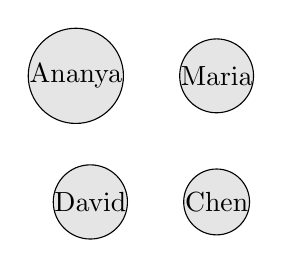
\begin{tikzpicture}
    	\node[main node,minimum size=0.8cm,fill={gray!20}] (v_{1}) {Ananya};
    	\node[main node,minimum size=0.8cm,fill={gray!20}] (v_{2}) [right = 0.7cm of v_{1}] {Maria};
		\node[main node,minimum size=0.8cm,fill={gray!20}] (v_{3}) [below = 0.7cm of v_{2}] {Chen};
    	\node[main node,minimum size=0.8cm,fill={gray!20}] (v_{4}) [left = 0.7cm of v_{3}] {David};    
    	
    \end{tikzpicture}
\hspace{3em}
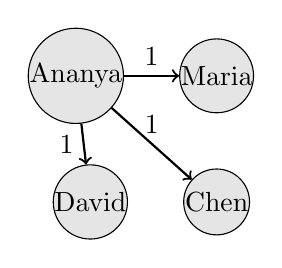
\begin{tikzpicture}
    	\node[main node,minimum size=0.8cm,fill={gray!20}] (v_{1}) {Ananya};
    	\node[main node,minimum size=0.8cm,fill={gray!20}] (v_{2}) [right = 0.7cm of v_{1}] {Maria};
		\node[main node,minimum size=0.8cm,fill={gray!20}] (v_{3}) [below = 0.7cm of v_{2}] {Chen};
    	\node[main node,minimum size=0.8cm,fill={gray!20}] (v_{4}) [left = 0.7cm of v_{3}] {David};
    
    	\path[draw,thick,->]
    	(v_{1}) edge node[midway,above] {$ {1} $} (v_{2})
    	(v_{1}) edge node[midway,above] {$ {1} $} (v_{3})
    	(v_{1}) edge node[midway,left] {$ {1} $} (v_{4});
    
    	
\end{tikzpicture}

\hspace{16em}

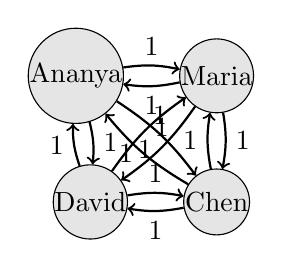
\begin{tikzpicture}
    	\node[main node,minimum size=0.8cm,fill={gray!20}] (v_{1}) {Ananya};
    	\node[main node,minimum size=0.8cm,fill={gray!20}] (v_{2}) [right = 0.7cm of v_{1}] {Maria};
		\node[main node,minimum size=0.8cm,fill={gray!20}] (v_{3}) [below = 0.7cm of v_{2}] {Chen};
    	\node[main node,minimum size=0.8cm,fill={gray!20}] (v_{4}) [left = 0.7cm of v_{3}] {David};
    
    	\path [->,bend left=10,thick]
    	(v_{1}) edge node[midway,above] {$ {1} $} (v_{2})
    	(v_{1}) edge node[right,above] {$ {1} $} (v_{3})
    	(v_{1}) edge node[midway,right] {$ {1} $} (v_{4})
    	(v_{2}) edge node[midway,below] {$ {1} $} (v_{1})
    	(v_{2}) edge node[midway,right] {$ {1} $} (v_{3})
    	(v_{2}) edge node[right,above] {$ {1} $} (v_{4})
    	(v_{3}) edge node[left,left] {$ {1} $} (v_{1})
    	(v_{3}) edge node[midway,left] {$ {1} $} (v_{2})
    	(v_{3}) edge node[midway,below] {$ {1} $} (v_{4})
    	(v_{4}) edge node[midway,left] {$ {1} $} (v_{1})
    	(v_{4}) edge node[midway,below] {$ {1} $} (v_{2})
    	(v_{4}) edge node[midway,above] {$ {1} $} (v_{3});
    
    	
    \end{tikzpicture}

\hspace{3em}
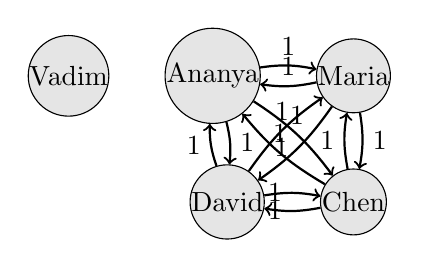
\begin{tikzpicture}
    	\node[main node,minimum size=0.8cm,fill={gray!20}] (v_{1}) {Ananya};
    	\node[main node,minimum size=0.8cm,fill={gray!20}] (v_{2}) [right = 0.7cm of v_{1}] {Maria};
		\node[main node,minimum size=0.8cm,fill={gray!20}] (v_{3}) [below = 0.7cm of v_{2}] {Chen};
    	\node[main node,minimum size=0.8cm,fill={gray!20}] (v_{4}) [left = 0.7cm of v_{3}] {David};
    	\node[main node,minimum size=0.8cm,fill={gray!20}] (v_{5}) [left = 0.7cm of v_{1}] {Vadim};
    
    	\path [->,bend left=10,thick]
    	(v_{1}) edge node[midway,above] {$ {1} $} (v_{2})
    	(v_{1}) edge node[midway,above] {$ {1} $} (v_{3})
    	(v_{1}) edge node[midway,right] {$ {1} $} (v_{4})
    	(v_{2}) edge node[midway,above] {$ {1} $} (v_{1})
    	(v_{2}) edge node[midway,right] {$ {1} $} (v_{3})
    	(v_{2}) edge node[midway,left] {$ {1} $} (v_{4})
    	(v_{3}) edge node[midway,above] {$ {1} $} (v_{1})
    	(v_{3}) edge node[midway,left] {$ {1} $} (v_{2})
    	(v_{3}) edge node[midway,left] {$ {1} $} (v_{4})
    	(v_{4}) edge node[midway,left] {$ {1} $} (v_{1})
    	(v_{4}) edge node[midway,above] {$ {1} $} (v_{2})
    	(v_{4}) edge node[midway,left] {$ {1} $} (v_{3});
    
    	
    \end{tikzpicture}
\hspace{3em}
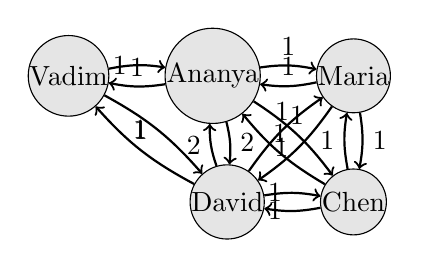
\begin{tikzpicture}
    	\node[main node,minimum size=0.8cm,fill={gray!20}] (v_{1}) {Ananya};
    	\node[main node,minimum size=0.8cm,fill={gray!20}] (v_{2}) [right = 0.7cm of v_{1}] {Maria};
		\node[main node,minimum size=0.8cm,fill={gray!20}] (v_{3}) [below = 0.7cm of v_{2}] {Chen};
    	\node[main node,minimum size=0.8cm,fill={gray!20}] (v_{4}) [left = 0.7cm of v_{3}] {David};
    	\node[main node,minimum size=0.8cm,fill={gray!20}] (v_{5}) [left = 0.7cm of v_{1}] {Vadim};
    
    	\path [->,bend left=10,thick]
    	(v_{1}) edge node[midway,above] {$ {1} $} (v_{2})
    	(v_{1}) edge node[midway,above] {$ {1} $} (v_{3})
    	(v_{1}) edge node[midway,right] {$ {2} $} (v_{4})
    	(v_{2}) edge node[midway,above] {$ {1} $} (v_{1})
    	(v_{2}) edge node[midway,right] {$ {1} $} (v_{3})
    	(v_{2}) edge node[midway,left] {$ {1} $} (v_{4})
    	(v_{3}) edge node[midway,above] {$ {1} $} (v_{1})
    	(v_{3}) edge node[midway,left] {$ {1} $} (v_{2})
    	(v_{3}) edge node[midway,left] {$ {1} $} (v_{4})
    	(v_{4}) edge node[midway,left] {$ {2} $} (v_{1})
    	(v_{4}) edge node[midway,above] {$ {1} $} (v_{2})
    	(v_{4}) edge node[midway,left] {$ {1} $} (v_{3})
    	(v_{5}) edge node[midway,left] {$ {1} $} (v_{1})
    	(v_{5}) edge node[midway,left] {$ {1} $} (v_{4})
    	(v_{1}) edge node[midway,above] {$ {1} $} (v_{5})
    	(v_{4}) edge node[midway,above] {$ {1} $} (v_{5});
    	
    \end{tikzpicture}
\caption{\textbf{Example of creating a social interaction graph between four GitHub developers.}
\textbf{Step 1 (LHS):} Ananya,Maria,Chen and David are four developers in a GitHub project. \textbf{Step 2:} Ananya creates one issue where Maria,Chen and David comment. So, we join Ananya-Maria,Ananya-Chen,Ananya-David with edge of weight 1. \textbf{Step 3:} A new developer Vadim comes. \textbf{Step 4 (RHS):} Vadim creates one new issue where Ananya and David comments. So, two new edges are introduced - (Ananya-Vadim(1), David-Vadim(1)).  Now we iterate for each developer, so all of them become connected and lastly,  weight of Ananya-David increases to 2.}
\label{fig:social_interaction_graph}       
\end{figure*}




\subsubsection{Product Metrics}
\label{sec:Product Merics}
This study explores the effects of social and code communication to assess code quality, by measuring the percentage of buggy commits introduced by developers (hero and non-hero developers),  but in order to do so we do need to identify the commits that introduced the bug in the code from the historic project data. This is   a 
challenging task since there is no direct way to find the commits or the person who is responsible for the bug/issue introduction. Hence,
our scripts proceed as follows:

\bi
\item
Starting with all the commits from {\tt git log},
we identify the commit messages.
\item
Next,  to use the commit messages for labeling,
we apply natural language processing~\cite{hindle2008large,rosen2015commit}
(to do  stemming, lemmatization and lowercase conversion to normalize the commit messages).
\item
Then to identify commit messages which are representation of bug/issue fixing commits, a list of words and phrases is  extracted from previous studies of 1000+ projects (Open Source and Enterprise). The system checked for these words and phrases in the commit messages and if found, it marks these as commits which fixed some bugs.
\item
To perform sanity check,  5\% of the commits was manually verified by 7 graduate students using random sampling from different projects. Disagreements between manual labeling and keyword based labeling was further verified and keywords were added or removed to improve performance.
\item
These labeled commits were then processed to extract the file changes as the process mentioned in process metrics section~\ref{sec:process metrics}.
\item
Finally,  {\tt git blame} is used to go back in the git history to identify a responsible commit where each line was created or changed last time.
\ei
By this process, commits that were responsible for introduction of the bugs in the system/project can be found. We label these commits as
``buggy commits'' and label the author of the commit as the ``person responsible'' for introducing the bug.






\subsubsection{Final Feature Extraction}
\label{sec:Finding Relation}
To assess the prevalence of
heroes in the software projects,  we joined across all the metrics shown above.
Specifically, using the two graphs,   we calculated the node degree (number of edges touching
a vertex) of the graphs
(and note that vertices with higher degree represent more communication or interaction). 

For the sake of completeness, we   varied our threshold of ``hero'' to someone belonging to  80\%, 85\%, 90\% and 95\% of the communication.  
In our studies,top contributors (or heroes) and non-heroes
 were defined as : 
\begin{equation}
\label{eq:node-Degree}
    \mbox{ Node Degree of } N_i = D(N_i)= \sum_{j=1}^{n} a_{ij}
\end{equation}
\begin{equation}
\label{eq:hero}
    \mbox{  Hero} = Rank\left(D(N_i)\right) > \frac{P}{100}*(N + 1)
\end{equation}
\begin{equation}
\label{eq:non-hero}
    \mbox{  Non-Hero} = Rank\left(D(N_i)\right) < \frac{P}{100}*(N + 1)
\end{equation}
where:


\begin{table}[h]
\centering
\begin{tabular}{|l|l|}
\hline
N & Number of Developers \\ \hline
P & 80,85,90 and 95 Percentile \\ \hline
Rank() & \begin{tabular}[c]{@{}l@{}}The percentile rank of a score is the percentage \\ of scores in its frequency distribution that is\\ equal to or lower than it.\end{tabular} \\ \hline
a & \begin{tabular}[c]{@{}l@{}}Adjacency matrix for the graph \\ where $a_{ij}>0$  denotes a connection\end{tabular} \\ \hline
\end{tabular}
\end{table}

Using these data and by applying the hero definition from formula (\ref{eq:hero}) and (\ref{eq:non-hero}) (look at the top 20\%,15\%,10\% and 5\%), we can find the developers who are responsible for 80\%,85\%,90\% and 95\% of the work. We use this to categorize the developers into 2 groups:
\bi
\item
The \textit{hero developers}; i.e. the core group of the developers of a certain project who make regular changes in the codebase. In this study this is represented by the developers whose node degree is above 80,85,90 and 95th percentile of the node degree (developers' communication and code interaction of the system graph).
\item
The \textit{non-hero developers} are all other developers;
i.e.  developers associated with  nodes with a degree below the respective threshold percentile.
\ei

Following this for each selected projects, we merge the product data collected in section~\ref{sec:Product Merics} and section~\ref{sec:process metrics} to find each developer's code contribution according to the code interaction graph. Similarly process is followed for  section~\ref{sec:Personnel Metrics} and section~\ref{sec:process metrics} in the social interaction graph. Using the above mentioned data, we can validate the code and social contribution of each developer along with their bug introduction percentage. This information will help us to answer the research questions asked in this study.

\section{Results}
\label{sec:Results}
Our results are structured around three research questions:
\begin{description}
    \item[{\bf RQ1:}] How common are hero projects?
    \item[{\bf RQ2:}] What    impact  does heroism  have  on  code quality?
    \item[{\bf RQ3:}] Does the results support Herbsleb Hypothesis?
    % \item[{\bf RQ4:}] Does the threshold of 80\% make sense?
\end{description}


\subsection*{\textbf{RQ1: \textit{How common are hero projects?}}}

Figure~\ref{fig:RQ1_following} shows the result for number of projects marked as hero and non-hero when the we vary the threshold from ``hero-ness''
from 80 to 95\%.The clear conclusion from this figure is
 that the phenomenon  that we have defined as ``hero``
 is very common. In fact, the phenomenon
 may be more pronounced than previously reported.
 Even when we say heroes are involved in 95\% of
 the communication, we find that that majority of the
 projects studied here exhibit ``hero-ness''. That is:

\begin{result}
Hero projects are overwhelmingly present in open source software community. That is, in the usual case,
 there are very few people in each project responsible for majority of the work.
\end{result}

 

\begin{figure}
\includegraphics[width=\linewidth]{RQ1_Code.png}
\caption{RQ1 Result: Distribution of hero projects vs non-hero projects based on hero threshold being 80\%, 85\%, 90\% and 95\% respectively. Here threshold being 80\% means in that project 80\% code is done by less than 20\% of developers}
\label{fig:RQ1_following}
\end{figure}


\subsection*{\textbf{RQ2: \textit{What impact does heroism have on code quality?}}}

RQ2 explores effect heroism have on code quality. In this study, we created the developer social interaction graph and developer code interaction graph, then identified the developer responsible for introducing those bugs into the codebase. Then we find the percentage of buggy commits introduced by those developers by checking (a)~the number of buggy commits introduced by those developers and (b)~their number of total commits.

Fig~\ref{fig:RQ2_code} and Fig~\ref{fig:RQ2_social}
shows the comparison between the performance of hero and non-hero developers. In those figures:
\bi
\item
The x-axis is different projects used in this study.
\item
The y-axis represents the median of the bug introduction percentage for all hero and non-hero developers for each project respectively.
\ei

\begin{figure}[!t]
\begin{center}
\includegraphics[width=.7\linewidth]{80_Code.png}
\includegraphics[width=.7\linewidth]{90_Code.png}
\includegraphics[width=.7\linewidth]{95_Code.png}
\end{center}
\caption{Code interaction  graph results for
RQ2: Percentage of bugs introduced by hero and non-hero developers from developer code interaction perspective in Hero Projects .}
\label{fig:RQ2_code}
\end{figure}

Here projects are sorted by the no. of non-hero developers. In those charts we note that:
\bi
\item
There exists a large number of non-heroes who always produce buggy commits, 100\% of the time (evidence: the flat right-hand-side regions of the non-hero plots in both figures). That population size of ``always buggy'' is around a third in 
Fig~\ref{fig:RQ2_code} and a fourth in Fig~\ref{fig:RQ2_social}.
\item
To say the least, heroes nearly always have fewer buggy commits than non-heroes. The 25th, 50th, 75th percentiles for both groups are
shown in table~\ref{tbl:team_size}. This table clearly shows why heroes are so  prevalent, they generate commits that are dramatically
less buggy than non-heroes, regardless of the size of the project.
\ei



\begin{figure}[]\begin{center}
\includegraphics[width=.7\linewidth]{80_Social.png}
\includegraphics[width=.7\linewidth]{90_Social.png}
\includegraphics[width=.7\linewidth]{95_Social.png}
\end{center}
\caption{Social interaction  graph results for
RQ2: Percentage of bugs introduced by hero and non-hero developers from developer social interaction perspective in Hero Projects.}
\label{fig:RQ2_social}
\end{figure}


\begin{table}[!t]
\caption{The table summarizes of Fig~\ref{fig:RQ2_code}, Fig~\ref{fig:RQ2_social} and stratifies the data according to 25th, 50th and 75th percentile of the developers.}
\label{tbl:team_size}
%{\scriptsize
\begin{center}
\begin{tabular}{|c|c|c|c|c|}
\hline
\rowcolor[HTML]{EFEFEF} 
\textbf{}                                     & \textbf{}         & \multicolumn{3}{c|}{\cellcolor[HTML]{EFEFEF}\textbf{Percentile}} \\ \hline
\rowcolor[HTML]{EFEFEF} 
\textbf{Metric}                               & \textbf{Group}    & \textbf{25th}        & \textbf{50th}       & \textbf{75th}       \\ \hline
                                              & \textbf{Hero}     & 0.52                 & 0.58                & 0.53                \\ \cline{2-5} 
                                              & \textbf{Non-Hero} & 0.67                  & 0.75                 & 1.0                 \\ \cline{2-5} 
\multirow{-3}{*}{\textbf{Code Interaction}}   & \textbf{Ratio}    & 1.3                  & 1.3                 & 1.9                 \\ \hline
                                              & \textbf{Hero}     & 0.44                  & 0.5                 & 0.5                 \\ \cline{2-5} 
                                              & \textbf{Non-Hero} & 0.67                 & 0.75                & 0.67                \\ \cline{2-5} 
\multirow{-3}{*}{\textbf{Social Interaction}} & \textbf{Ratio}    & 1.5                  & 1.5                 & 1.3                 \\ \hline
\end{tabular}
\end{center}%}
\end{table}


The other thing to note from 
Fig~\ref{fig:RQ2_code} and Fig~\ref{fig:RQ2_social}
is that they are nearly identical.
That is, no matter how we define ``hero'',
we reach the same conclusions.
Hence we say -  

\begin{result}
In modern software projects,
 reflecting on
  who writes most of the code is just as insightful
  as reflecting on  who participates in most
of the discussion about the code.
\end{result}

\subsection*{\textbf{RQ3: \textit{Do the results support Herbsleb Hypothesis?}}}

In this RQ, we explored the Herbsleb hypothesis~\cite{Herbsleb:2014} from section~\ref{sec:Background And Prior Work}; i.e. does lack of communication between developers predict for bugs in the code? In order to do that for 1,037 projects, we discretized the developers into 3 groups (i.e. High, Medium and Low) based on their code contribution (Code Node Degree) and social communication frequency (Social Node Degree). In Figure~\ref{fig:Herbsleb_stats}, group HH (High,High) represents the developers who have high high code contribution and social communication frequency and the value in the cell is median bug introduction percentage, while group LL (Low,Low) represents the developers who have low code contribution and low social communication frequency. 

Figure~\ref{fig:Herbsleb_stats} shows the result of statistical test performed on the 9 different groups representing different frequency and volume of communication. We can see from this figure group LH, LM and LL are in different ranking representing  the median bug introduction be these groups are statistically significantly different. Same can be seen for MH, MM and ML groups. While HH, HM and HL has same ranking representing the median bug introduction be these groups are not statistically significantly different. This findings shows the groups where developers are doing low to medium code contribution, communication is an very important factor (i.e. LH, LM and LH shows the bug introduction increases from 30\% , 38\% and 67\% respectively). These results support the Herbsleb hypothesis, which suggests communication between developers is an important factor and lesser social communication can lead to more bugs.




\begin{figure}[!t]
\centering
{\small
{\small \begin{tabular}{llrrc}
\arrayrulecolor{darkgray}
\rowcolor{darkgray}  rank & group & median & IQR & \\
\rowcolor{blue!10}    1 &      LH &    30 &  29 & \quart{18}{30}{29}{17} \\
\rowcolor{gray!20}    1 &      MH &    38 &  28 & \quart{26}{38}{28}{16} \\
\rowcolor{blue!10}    2 &      LM &    38 &  31 & \quart{25}{38}{31}{18} \\
    2 &      HH &    42 &  18 & \quart{33}{42}{18}{9} \\
\rowcolor{gray!20}    2 &      MM &    46 &  21 & \quart{35}{46}{21}{10} \\
    2 &      HM &    46 &  21 & \quart{33}{46}{21}{8} \\
    2 &      HL &    48 &  30 & \quart{34}{48}{30}{16} \\
\rowcolor{gray!20}    3 &      ML &    52 &  29 & \quart{38}{52}{29}{15} \\
\rowcolor{blue!10}    4 &      LL &    67 &  55 & \quart{45}{67}{55}{33} \\
\end{tabular}}
}
\caption{This figure shows the result of statistical significance test and an effect size test on 9 different groups used to study the Herbsleb hypothesis. In this figure the group column represents the 9 different groups in this research question, where the first character represents the code node degree, while the later is social node degree.
}
\label{fig:Herbsleb_stats}
\end{figure}
%%%%%%%%%%%%%%

This finding leads to  the following
conjecture (to be explored
in future work):
the best way to reduce communication overhead and to decrease defects is to {\em centralize the communicators}. In our data, commits with lower defects come from the small number of hero developers who have learned how to talk to more people. Hence, we would encourage more research into better methods for rapid, high-volume, communication in a one-to-many setting (where the ``one'' is the hero and the ``many'' are everyone else). In summary, we can say 

\begin{result}
The Herbsleb hypothesis holds true for open source software projects. More research should be performed to find better methods for rapid, high-volume, communication in a one-to-many setting.
\end{result}

% \subsection{\textbf{RQ4:} \textit{Does the threshold of 80\% make sense?}}
% \label{sec:RQ4}

% In this RQ we try to verify if the default threshold for defining heroes, that is 80\% of the work is done by 20\% of the developers. We specifically explore the projects with varying definition of heroes, where increase the amount of work done from 80\% to 95\% and decrease the number of person involved from 20\% to 5\%. We can see from fig~\ref{fig:RQ1_following}, when we increase the threshold for defining a project as hero projects, till 90\%-10\% threshold most of the projects are hero projects, that means in more than 90\% of the projects that we validated 90\% or more work was done by 10\% or less developers. Even when the threshold is raised to 95\%-5\% almost 60\% of the projects can be defined as hero projects. This shows the prevalence of hero and amount of work they actually perform is much more than anticipated in open source community than previous literature.
% We can also see from the fig~\ref{fig:RQ2_code} and fig~\ref{fig:RQ2_social} with the varying definition of heroes the graph doesn't change much, both communication ans code graphs shows the average bug introduction rate by hero developers are much less than non-hero developers. With these results we can see the amount of work done by developers almost follows power law distribution, which is a natural occurrence and is prevalent in open source software projects.


\section{Discussion}
\label{sec:Discussion}

\subsection{Chief Programmer}
One strange feature of our results is that what is old is now new.   Our results (that heroes are important) echo a decades old concept. In 1975, Fred Brooks wrote of  ``surgical teams'' and the ``chief programmer'' ~\cite{brooks1974mythical}. He argued that - 

\begin{itemize}
  \item  Much as a surgical team during surgery is led by one surgeon performing the most critical work, while directing the team to assist with less critical parts.
  
  \item Similarly, software projects should be led by one ``chief programmer'' to  develop critical system components while the rest of a team provides what is needed at the right time.
\end{itemize}
Brooks conjecture that ``good'' programmers are generally much more as productive as mediocre ones. This can be seen in the results that hero programmers are much more productive and less likely to introduce bugs into the codebase.
Heroes are born when developers become are so skilled at what they do, that  they assume a central position in a project.
In our view,  organizations need to acknowledge their dependency on such heroes, perhaps altering their human resource policies and manage these people more efficiently by retaining them.

\subsection{Power Law}
Throughout the years, empirical studies have found power law distributions in various measures across many software systems~\cite{louridas2008power,concas2007power,wheeldon2003power,lin2015power,madey2002open}. The abundance of open source software repositories allows researchers to  analyze software systems and their evolution, which reveals the prevalence of similar distributions in software: in change sizes, in-degree and out-degree in dependency network, number of sub classes, and so on. Lin et al.~\cite{lin2015power} argued in their paper - 

``In fact, if one were to analyze the distribution of another measure of software, it would be most surprising to find it not following a power law or other heavy-tailed distribution.''

This study finds power law distribution in code communication and social communication between developers while analyzing over 1000+ projects.


\section{Threats to Validity}
\label{sec:Threats to Validity}
  \subsection{Sampling Bias} Our conclusions are based on 1000+ open source GitHub projects that started this analysis.  It is possible that   different initial projects would have lead to different conclusions. That said, our initial sample is very large so we have some confidence that this sample represents an interesting range of projects.  
            
     \subsection{Evaluation Bias} In  RQ1,RQ2 and RQ3, we said that heroes are prevalent and responsible for far less bug introduction than non-hero developers.
     It is possible that, using other metrics like if heroes reduce productivity by becoming bottleneck, there may well be a difference in these different kinds of projects. But measuring people resources only by how fast releases are done or issues are fixed may not be a good indicator of measuring affects of having heroes in team. This is a matter that needs to be explored in future research. 

         \subsection{Construct Validity} At various places in this report, we made engineering decisions about (e.g.) team size; and (e.g.) what constitutes a ``hero'' project. While those decisions were made using advice from the literature (e.g.~\cite{gautam2017empirical}), we acknowledge that other constructs might lead to different conclusions. 
     

\subsection{External Validity} 
In the literature, ``hero developers'' are those who are responsible for 80\% of the work. In our study, we try with 80\%, 85\%, 90\% and 95\% threshold and get the same conclusion that majority of our sample projects are hero-dominated. Here we do not contradict with the prior definition of heroism, we rather verify it with different thresholds.


We have relied on natural language processor to analyze commit messages to mark them as buggy commits. These commit messages are created by the developers and may or may not contain proper indication of if they were used to fix some bugs. There is also a possibility that the team of that project might be using different syntax to enter in commit messages.

Similarly we have used GitHub issues and comments to create the communication graph, It is possible that the communication was not made using these online forums and was done with some other medium. To reduce the impact of this problem, we  did take precautionary step to (e.g.,) include various tag identifiers of bug fixing commits, did some spot check on projects regarding communication etc.

Our conclusion shows that almost all (when experimenting with 80\%, 85\%, 90\% threshold) of our sample projects are hero dominated.  In case of large size public GitHub projects, there are official administrators and maintainers who are responsible for issue labelling or assigning. So, they frequently comment on all of the issues but though they are not active developers. These people should not be considered as hero developers. Finding these people needs manual inspection which is not possible for 1000+ projects. We decide to put it as a limitation of our study as we deal with a huge no. of projects.

We do not isolate hero projects and non-hero projects and look into them separately because there are very few non-hero projects and also there are a lot of developers who work in a large no. of projects (some of them are hero projects and some of them are not). We have sample bias that we did not find any hero related papers in recent high profile software engineering conferences. We have looked for such papers but did not find any in the last five years. We have evaluation bias as we report cumulative statistics of lift curves where other papers reported precision and recall. The research in this field is not mature enough yet for us to say that the best way to represent results is one way vs. the other. Here we decided to use lift curves. We note that if we did use precision and recall, we had to repeat that analysis at multiple points of the lift curve. We find our current lift curves are a succinct way to represent our results. One threat to construct validity that we did not consider the different roles of the developers. We had trouble extracting that information from our data source, we found that people have multiple roles particularly our heroes who would often step in and assist in multiple activities.  Nevertheless the exploration of different roles would be an interesting study to do. Previously Agrawal et al. were able to compare open and closed source projects. That research group was fortunate enough to work on-site at a large open source software company. We were not as fortunate as them. We therefore acknowledge our findings may not be the same for closed source projects. Having said that we do mention that our conclusions match with their findings as nearly all projects are hero-based projects.


 

 
\section{Conclusion}
\label{sec:Conclusion}

The established wisdom in the literature is to depreciate ``heroes'',
i.e., a small percentage of the staff who are responsible for most of the progress on a project.
But, based on a study of 1000+ open source GitHub projects,
we assert:
\bi
\item  Overwhelmingly, most projects are hero projects.
\item   Hero developers are far less likely to introduce bugs into the codebase than their non-hero counterparts. Thus having heroes in projects significantly affects the code quality.
\ei
Our empirical results call for a revision of a long-held truism in software engineering.
Software heroes are far more common and valuable than suggested by the literature,
particularly from code quality perspective. Organizations should reflect on better ways
to find and retain more of these software heroes.

More generally, we would  comment that  it is time
to reflect more on long-held truisms in our field. Heroes are widely deprecated in the literature, yet empirically they are quite beneficial. 
 What other statements in the literature need to be
reviewed and revised?




% \balance
\bibliographystyle{plain}
\bibliography{Mybib}

\end{document}
\endinput
%%
%% End of file `sample-acmtog.tex'.
